\chapter[Solução Proposta]{Solução Proposta}


\section{Dimensionamento do Forno}

O forno de tratamento térmico possuirá um volume interno de aproximadamente 8 litros, pois o objetivo é fabricar um forno de tratamento para fins acadêmicos, com corpos de prova segundo a norma ABNT 10611 e componentes mecânicos de pequeno porte, como engrenagens.
 
A parte externa será compostas por uma estrutura de aço carbono como um chassi de sustentação ao peso do forno bem como todo suporte para materiais elétricos/eletrônicos, esse envoltório também será usado em formato de placas de para cobrir os tijolos expostos ao ambiente externo a fim de proteger contra choque mecânicos, conforme demonstrado no anexo b.

Os tijolos utilizados para tal construção possuem dimensões de 350 x 150 x 60 (mm) e são próprios para suportar temperaturas superiores a 1200 ºC conforme mostrado na tabela a seguir, concedida pela empresa fornecedora desse material.

\begin{figure}[!ht]
	\centering
	\label{tabela_dimensoes}
	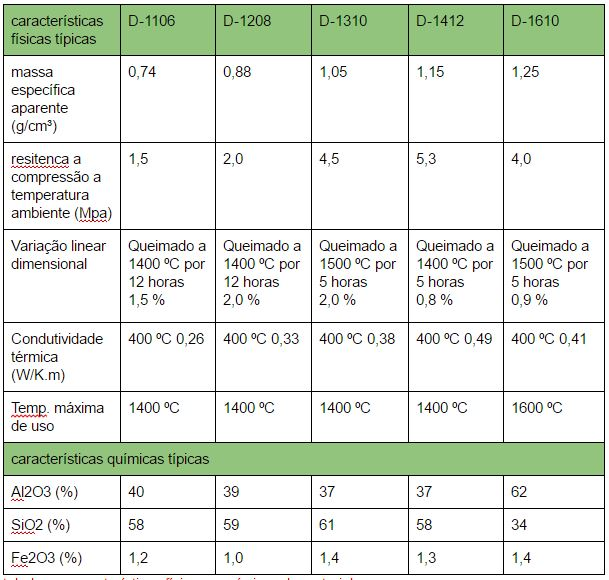
\includegraphics[keepaspectratio=true,scale=0.7]{figuras/tabela_dimensoes.JPG}
	\caption{Características físicas e químicas do material.}
\end{figure}

\subsection{Definindo alguns parâmetros de medida dentro do forno para definir os requisitos não funcionais}

Como ponto de partida, foi considerado um forno pequeno para o tratamento térmico de um corpo de prova de aço. Este corpo de prova será submetido a uma temperatura de $1200\degree C$, afim de se introduzir a martensita em sua estrutura, que é responsável pelo endurecimento e aumento da rigidez na estrutura do aço.

Para o forno térmico, será então calculado algumas propriedades técnicas de funcionamento do forno, a espessura do isolante térmico selecionado, a temperatura máxima de operação da parede interna, onde as resistências serão instaladas, a temperatura máxima nas paredes sem a fonte de calor instalada, ou seja, várias incógnitas muito importantes na hora da montagem do produto

A seguir é apresentado em uma tabela algumas constantes consideradas para a primeira análise dessas propriedades. Na qual estão presentes alguns valores necessário para o cálculo das propriedades previstas no parágrafo anterior.


\begin{figure}[!ht]
	\centering
	\label{tab_constantes}
	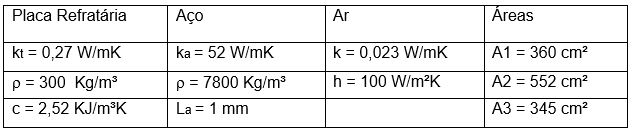
\includegraphics[keepaspectratio=true,scale=1.0]{figuras/tab_constantes.JPG}
	\caption{Tabela de propriedades técnicas.}
\end{figure}

\begin{figure}[H]
	\centering
	\label{vol_interno}
	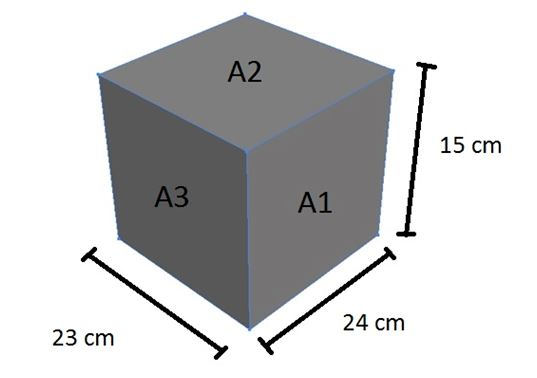
\includegraphics[keepaspectratio=true,scale=0.8]{figuras/vol_interno.JPG}
	\caption{Dados do Volume Interno do Forno.}
\end{figure}

A imagem acima retrada o dimensionamento interno escolhido pelo grupo de trabalho, onde A3 será a entrada do forno e terá área igual ao fundo, A1 e A2 são os lados, base e fundo respectivamente. . 

\section{Cálculo da distribuição de temperatura no interior do forno}

Nesta seção será tratado sobre os mecanismos básicos da condução de calor, convecção, condução e radiação. Estes ocorrem dentro do forno, através principalmente pela diferença de temperatura entre o interior do forno e o meio ambiente, que geram um fluxo de calor na direção do mais quente para o mais frio.

O cálculo desse fluxo de calor por meio da condução, convecção e radiação se dá pelas seguintes fórmulas.



******

formulas

******


\begin{figure}[H]
	\centering
	\label{dist_temperatura}
	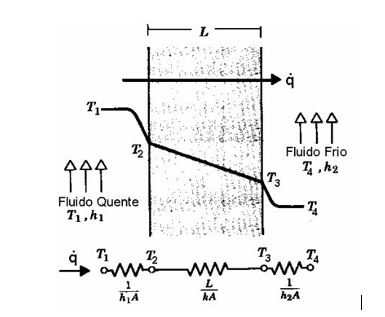
\includegraphics[keepaspectratio=true,scale=0.8]{figuras/dist_temperatura.JPG}
	\caption{Distribuição da temperatura ao longo de um material.}
\end{figure}

\begin{figure}[H]
	\centering
	\label{dist_temperatura}
	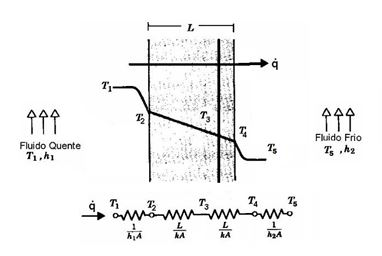
\includegraphics[keepaspectratio=true,scale=1.0]{figuras/dist_temperatura2.JPG}
	\caption{Distribuição da temperatura ao longo da porta e do fundo.}
\end{figure}

Para o Cálculo do coeficiente de radiação, foi preciso fazer algumas considerações. É considerado que as resistências estão na sua temperatura de trabalho, um grau a mais que na temperatura ambiente enquanto que o meio está em sua temperatura ambiente inicial, ou seja, enquanto o ambiente estiver no máximo a $1200\degree C$, as resistências estarão a $1201\degree C$ e o meio a $27\degree C$. 

Além disso, este cálculo foi feito apenas para as resistências que possui a emissividade de 0,7, e não para o interior das placas refratárias, por essas possuírem um baixo valor de emissividade de 0,29, e ser necessário um processo iterativo de cálculo, a qual não se faz necessário para uma primeira estimativa.

Com isso, a partir da fórmula do coeficiente de radiação, foi calculado o seguinte valor para o coeficiente de radiação.
*********formula*********

Com isso tudo esclarecido será calculado a temperatura nas paredes internas no forno e as espessuras da camada isolante do forno, considerando os materiais escolhidos (Tijolo refratário e o aço carbono).

Considerando o primeiro trecho, partindo do interior com 1200ºC até a parede interna com as resistências instaladas, a fórmula para o cálculo da temperatura, será apresentado logo a seguir.

Foi considerado as paredes laterais do forno, a base e o topo como tendo resistências, a temperatura nessas paredes, em A1 e A2 será a seguinte.

*********

formula

**********

Além disso foi considerado que as resistências estão igualmente espaçadas nas 4 paredes, ou seja, a potência também será dividida e sendo considerada como 750 W em A1 e A2.

\begin{figure}[H]
	\centering
	\label{form3}
	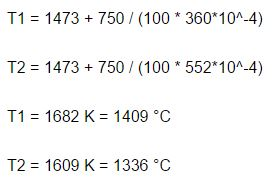
\includegraphics[keepaspectratio=true,scale=1.0]{figuras/form3.JPG}
\end{figure}


As temperaturas nas superfícies A3 (forno e porta), serão consideradas, iguais as temperaturas de operação do forno, para se adquirir um sobre dimensionamento da espessura requerida para os tijolos refratários, então T3 será igual a $1200\degree C$. Em outras palavras, foi considerado que não há problema algum de isolamento no fundo e na porta do forno, ou seja, nenhuma energia estaria se dissipando.

Com as temperaturas nas paredes bem definidas, é possível calcular a transferência de calor nos tijolos refratários e nas placas de aço carbono, considerando apenas o fenômeno da condução.

*******

formula

*******

 A única variável são as áreas que dependem da seção analisada e a espessura do tijolo. Por vias de uma segurança maior nos cálculos, serão considerados a temperatura na placa externa igual a temperatura no meio ambiente de 27ºC. A equação simplificada para obter Lt é a seguinte.
 
********

formula


*******
 
Os cálculos com os subscritos x, são correspondentes com as seções analisadas. Cada uma delas com uma área e diferença de temperaturas diferentes, e consequentemente terão espessuras requeridas diferentes. A Potência correspondente para cada seção será novamente de 750 W devido a uma divisão homogênea dos resistores nas seções consideradas.
 
*****

formula

********

\begin{figure}[H]
	\centering
	\label{tab}
	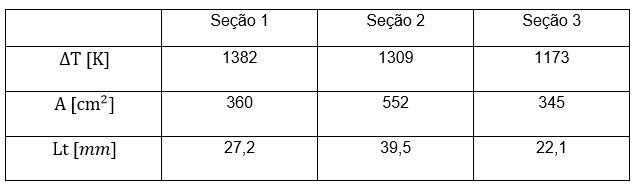
\includegraphics[keepaspectratio=true,scale=1.0]{figuras/tab.JPG}
	\caption{Cálculo das variáveis de temperatura interna do forno.}
\end{figure}

As espessuras requeridas para o tijolo refratário selecionado, foram calculadas. Este caso não leva em conta a dissipação de calor entre os tijolos. Afim de se ter tal valor, seria necessária fazer uma análise mais apurada experimentalmente ou numericamente.
Devido a todos os tipos de perdas de calor que possam ocorrer, é necessário um fator de segurança nessas espessuras obtidas. 

Além disso pode ser acrescentado algum material isolante entre os tijolos e as placas externas de aço, como a vermiculita.
Por fim, também tem os sulcos que serão feitos nos tijolos para o encaixe das resistências, este fator acarretara uma perca de material refratário, sendo necessário por fins de segurança, um aumento das espessuras calculadas.

\subsection{Cálculo das Potências dissipadas dentro do forno em cada seção}
As áreas das seções do forno foram definidas anteriormente, o objetivo dessa seção é saber o valor quantitativo de potência dissipada dentro do forno afim de se ter uma distribuição mais homogênea possível de calor dentro do forno.

Um dado obtido anteriormente neste trabalho é o tamanho necessário de resistência dentro do forno para alimentar o forno com uma potência de 3kW. Esse valor era de 30,73 metros, porém depois de comprar essa resistência e medir o comprimento real para obtermos 3 kW em uma tomada qualquer de 220 V, o seu novo comprimento foi de 26 metros.

Com base nesse novo valor de comprimento, será realizado o cálculo dos comprimentos das resistências nas seções 1 e 2. Mas antes por proporção de área, será calculado as áreas superficiais de resistências, para que elas fiquem igualmente distribuídas nessas 2 seções.

Declarando as variáveis X1 e X2 como sendo essas áreas superficiais equivalentes de resistência instaladas nas seções 1 e 2 respectivamente, temos os seguintes valores para X1 e X2.

**********

formulas

************

Com esses valores podemos calcular os comprimentos dos fios localizados nas seções 1 e 2 da seguinte maneira.

**********

formulas

************

Com esses valores, é possível calcular o valor das resistências nas seções 1 e 2, pois sabe se que 26 m equivale a $16 \Omega$, portanto o fio deste projeto possui uma densidade resistiva de $0.6154 \Omega /m$, resultando nos seguintes valores para R1 e R2.

**********

formulas

************

Com o valor da corrente de i = 13,63 A, é possível calcular a potência dissipada portanto nas seções 1 e 2.

**********

formulas

************

Por fins de praticidade, será calculado o valor da potência dissipada pela resistência em apenas 1 parede de cada sessão e o seu comprimento, pois este dado será utilizado na simulação no ANSYS. Esses valores são os seguintes.

**********

formulas

************

\section{Sistema de Alimentação}

\subsection{Tipo de Alimentação}

O sistema de aquecimento do forno para tratamento térmico pode ser por meio convectivo com queimadores de alta velocidade com ar quente através da queima de gás GLP ou gás natural, ou o aquecimento pode ser através de resistências elétricas de alta temperatura. 

Os queimadores são convenientemente dispostos e aproximados para que possam atingir a taxa de temperatura adequada, porém há vários fatores que indisponibilizam essa tecnologia, já que não há um isolamento entre as chamas e o material a sofrer tratamento térmico, o controle da temperatura seria um grande desafio. A segurança é outro fator muito importante, visto que o seu uso torna o sistema quanto ao manuseio periculoso. O fator recurso financeiro também foi levantado em consideração, já que há uma a indisponibilidade do recurso na Unidade Acadêmica de Ensino.

O aquecimento resistivo é largamente empregado devido ao baixo custo e à boa confiabilidade quando comparado a outros métodos de tratamento térmico localizado. Consiste de elementos resistivos convenientemente ajustados em torno do local a ser tratado; o conjunto é protegido por mantas cerâmicas, material de isolação térmica capaz de manter a região tratada sob temperaturas de até $1200\degree C$.

Como requisitos de segurança do sistema e da rede que conecta a tomada, o sistema será dimensionado para até 15 Amperes de corrente, pois de acordo com a NBR 14136, as tomadas domésticas devem operar a uma corrente de até 20 Amperes. Fazendo um fator de segurança de 5 amperes evitamos vários problemas com a sobrecarga do circuito.

\subsection{Sistema de Aquecimento}

Para que o interior do forno de tratamento térmico atinja altas temperaturas, serão usados resistores para a geração de calor, os quais serão conectados a fonte de tensão a partir de um circuito de controle de corrente e estarão posicionados nas paredes internas do forno. Tais resistores se comportarão como fontes de calor para atmosfera interna do forno, e estarão dispostos de forma que tenha a maior área possível de contato para o ar e que exista um caminho livre para circulação e transferência do calor.

Pela lei de ohm $(V=R x I)$, consegue-se garantir uma corrente constante e abaixo da estabelecida pela norma. Para que a temperatura seja controlada dentro do forno, será construído um circuito controlador, que fará uma flutuação entre na corrente, mantendo a temperatura dentro do forno com a menor flutuação possível.

\subsection{Cálculo de Potência e Tempo de Aquecimento}

Para alcançar a potência desejada de 3kW dimensionou-se as propriedades termodinâmicas no volume de controle do forno.

Para definir a Potência, julgou-se uma situação de alta quantidade de calor necessária para esquentar um corpo de prova cujo tamanho seja igual ao volume interno do forno e de temperatura de têmpera alta, próxima ao definido pelo escopo do projeto que é um forno que atinja 1200ºC. O material escolhido foi o Aço rápido sinterizado ASP 2017. Segue abaixo a curva de transformação com resfriamento contínuo do aço citado [11].
\begin{figure}[!h]
	\centering
	\label{transf_continuo}
	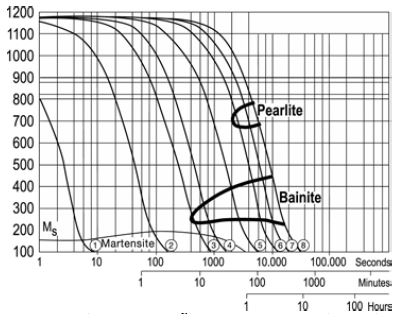
\includegraphics[keepaspectratio=true,scale=0.8]{figuras/transf_continuo.JPG}
	\caption{Curva de transformação com resfriamento contínuo.}
\end{figure}

\begin{align}
	T_{temp} = 1180 \degree C
\end{align}

A quantidade de calor necessária para aquecer a temperatura de têmpera do Aço rápido sinterizado ASP 2017 está diretamente relacionada às suas propriedades como $Ttemp=1180ºC$, sua massa específica $p = 8000 kg/m^{3}$  
e seu calor específico $c = 420 J/KgºC$ (Referência) não variando com a Temperatura, pela fórmula abaixo:

\begin{align}
	Q = \rho * V * c * (T_{temp} - T_{amb})
\end{align}

Sendo V o volume de aproximadamente 8,28 litros, a	 Tamb=20ºC, substituindo na fórmula temos:

\begin{align}
Q &= 8*10^{3}*8,28*10^{-3}*420*(1180-20) \\
\nonumber
Q &= 32,3 MJ
\end{align}

A partir dessa proposição e de acordo com a Primeira Lei da Termodinâmica para balanço de energia, e considerando o sistema adiabático de dentro do forno para o meio externo, a quantidade de calor Q é igual ao trabalho elétrico Wel convertido em energia térmica no meio. Sendo assim o balanço de energia se dá como:

\begin{align}
Q &= W_{el}
\end{align}

Possuindo o Wel, conseguimos relacionar a Potência necessária para o forno, através da fórmula:

\begin{align}
P &= \frac{W_{el}}{\Delta t}
\end{align}

Sendo P a potência e $\Delta$ t o tempo em segundos. 

Supondo uma Potência de 3 kW, e achando o tempo necessário:

\begin{align}
\Delta t &= \frac{W_{el}}{P} = \frac{32,3*10^6}{3*10^3} = 10758seg = 2,98h
\end{align}

Portanto, para aquecer um corpo de prova em uma situação de alta exigência do forno, o tempo de 3 horas é julgado aceitável para o projeto.

\subsection{Dimensionamento da Resistência Elétrica}

Para calcular a resistência foi utilizada a seguinte fórmula:

\begin{align}
R = \frac{V^2}{P}
\end{align}

Em que a tensão utilizada é de 220V e a potência é de 3kW. Feito os cálculos, a resistência encontrada foi de $16,13 \Omega$. Estas serão as condições para calcular a corrente máxima, onde o forno chegará a temperaturas de 1200 C. Para o material foi escolhido o fio Kanthal A-1(Cr 22\%, Al 5.8\% e Fe 72.2\%), levando em consideração a durabilidade e o alto desempenho desse material. Sabendo que o valor da resistência varia de acordo com a temperatura, é necessário converter essa resistência de acordo com a temperatura ambiente. Para valores de corrente e resistência, utilizou-se a temperatura de 20ºC, da seguinte forma:

\begin{align}
R_{20\degree C} = \frac{R(T)}{C_T(T)}
\end{align}

Onde $R(T)=16,13\Omega$ e $CT(T)=1,04$, que é o fator de conversão do material a $1200\degree C$. Obtendo $R_{20\degree C}=15,5\Omega$.

Utilizando os fatores de conversão do material, é possível determinar a variação da resistência com o aumento da temperatura. A tabela a seguir apresenta esses valores:

\begin{figure}[H]
	\centering
	\label{tabela1}
	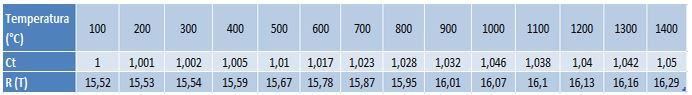
\includegraphics[keepaspectratio=true,scale=0.9]{figuras/alimentacao0.JPG}
\end{figure}
\begin{figure}[!h]
	\centering
	\label{grafico1}
	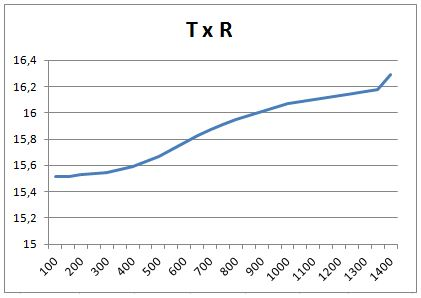
\includegraphics[keepaspectratio=true,scale=0.8]{figuras/alimentacao0_1.JPG}
	\caption{Gráfico 1:  Resistência em relação a temperatura}
\end{figure}

Observa-se a partir do gráfico acima, que a resistência aumenta com o aumento da temperatura, isso ocorre devido a degradação da  mobilidade de elétrons com o aumento da temperatura.

A corrente máxima que passa através do fio é dada por:

\begin{align}
I_{M\acute{A}X} = \frac{V}{R}
\end{align}

Utilizando V=220V e $R=16,13\Omega$ , obtém-se a corrente máxima de 13,64 A que está dentro da faixa de seguraça definida no projeto. Para escolher o fio mais apropriado que irá suportar essa corrente sem ser sobrecarregado foi calculada a superfície irradiante, que é calculada pela seguinte expressão:

\begin{align}
S_i = \frac{I_{M\acute{A}X}^{2}*C_T(T)}{\gamma}
\end{align}

Substituindo $I_{M\acute{A}X}=13,64A$, $C_T(T)=1,04$ e $y=2W/cm^{2}$(capacidade de condução de corrente), tem-se $96,75 cm^{2} / \Omega$. Pelas tabelas Kanthal, o fio mais apropriado, cuja superfície irradiante se encontra mais próxima desse valor, é o fio Kanthal A-1 com diâmetro 1,80mm e resistividade de $0,546\Omega /m$. O comprimento do fio é calculado pela expressão:

\begin{align}
I= \frac{R_{20 \degree C}}{0,546}
\end{align}

O comprimento encontrado foi de 28,41m.

\subsection{As resistências para aquecimento do forno}

Após os cálculos do dimensionamento do sistema de alimentação, foi definido e justificado a escolha do fio Kanthal A-1 como o material da resistência a ser utilizado.
Buscou-se em seguida realizar a compra do mesmo para iniciar a montagem do forno. Dentre os orçamentos realizados, optamos por um em preço que se adaptaria com a forma de trabalho da equipe. Por exemplo, a compra de uma maior metragem de fio para se ter uma folga de trabalho e o mesmo não enrolado para economizar no gasto de mão de obra.
A partir dessa definição, optamos pela compra online da loja de materiais elétricos Casa Ferreira, situada em São Paulo. A resistência Kanthal A-1 nesta loja é vendida por quilo, e esse quilo totalizava 55 metros de fio. Tendo estimado o uso de cerca de 28 metros, sobra uma quantidade interessante de fio do ponto de vista de folga de trabalho. Sem a mão de obra de enrolar o fio embutida, encontrou-se um valor bem abaixo dos orçados em Brasília. Com o frete, o quilo de Kanthal A-1 saiu a R\$ 174,73.


\begin{figure}[!h]
	\centering
	\label{resistencia1}
	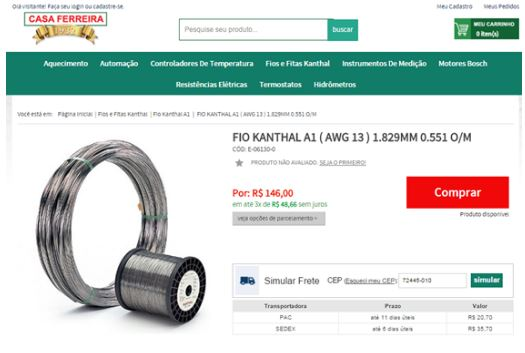
\includegraphics[keepaspectratio=true,scale=1.0]{figuras/alimentacao1.JPG}
	\caption{Valor das Resistências}
\end{figure}

\subsection{Distribuição das resistências no forno}

Para alocar as resistências dentro do forno de forma segura utilizamos a área interna das paredes do forno temos 3 dimensões:
\\Fundo e porta: $23x15 cm^2$
\\Laterais: $24x15cm^2$
\\Teto e base: $24x23cm^2$


As paredes da porta e do fundo não foram usadas para colocar as resistências porque a porta terá muito esforço mecânico impossibilitando as conexões da resistências além de diminuir a segurança do operador e o fundo será usado para colocar o termopar e será onde será ligada a alimentação das resistências. Para distribuição foi usado o espaço nas laterais no fundo e no teto.

Utilizamos uma distância mínima de 4 cm para a porta, 4 cm para a parede de fundo, e 2 cm de distância entre laterais e o fundo/topo. Assim a área que usamos usar para fazer as canaletas era:
\\laterais: $11x16cm^2$
\\fundo/topo: $19x16cm^2$

\begin{figure}[H]
	\centering
	\label{areaforno}
	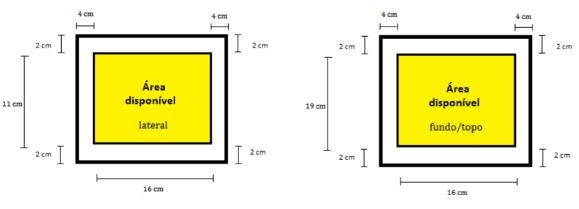
\includegraphics[keepaspectratio=true,scale=1.0]{figuras/alimentacao2.JPG}
	\caption{Área do Forno}
\end{figure}

Para calcular a largura da espira que contém n bobinas da resistência Kanthal A-1 precisamos dimensionar os parâmetros da espira como na figura a seguir:

\begin{figure}[H]
	\centering
	\label{areaforno}
	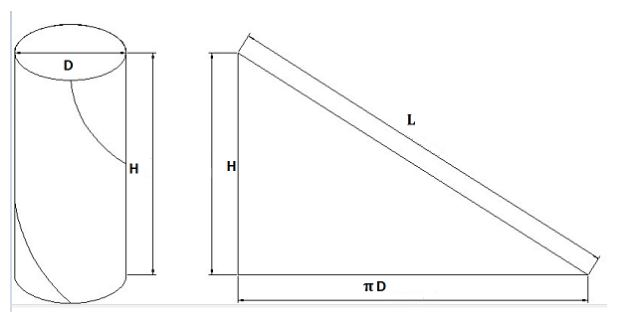
\includegraphics[keepaspectratio=true,scale=1.0]{figuras/alimentacao3.JPG}
\end{figure}

Para uma volta na bobina da resistência temos o diâmetro \textbf{D} da bobina, a altura \textbf{H} que corresponde a altura da espira e a largura do fio \textbf{L}. Abrindo a circunferência vemos que \textbf{L} é a hipotenusa do triângulo retângulo com \textbf{H} de um dos lados e a circunferência \textbf{$\pi D$} do outro.
Logo para \textbf{n} bobinas considerando a circunferência \textbf{$\pi D$} como valor fixo e a média da altura de cada bobina \textbf{H/n} como valor fixo bobina  a fórmula para dimensionar as propriedades da bobina é:

**********(formula)**********
******************

Considerando a expressão da altura de uma bobina \textbf{H/n=h} ou também chamado de “passo” e manejado as incógnitas temos uma expressão para o diâmetro da bobina:

**********(formula)**********
******************

Onde H é o comprimento total da espira, h é o passo, D é o diâmetro da bobina (diâmetro interno + raio do fio) e L é o comprimento total do fio.
Pelas medições precisávamos de uma resistência de $15,5\Omega$ (Ohm) o que dava uma média de 26 metros de comprimento de fio (L) usando o multímetro calibrado com o multímetro do laboratório de materiais da UnB gama.
Com o diâmetro da espira sendo o mínimo desejável para não se aprofundar muito na parede e ao mesmo tempo não ser pequeno ao ponto de diminuir a quantidade de resistência no área da parede vimos que o diâmetro seria por volta de 1,5 cm e com um espaço de segurança de no mínimo 2 cm entre uma canaleta e outra temos:

\begin{figure}[H]
	\centering
	\label{resistencia2}
	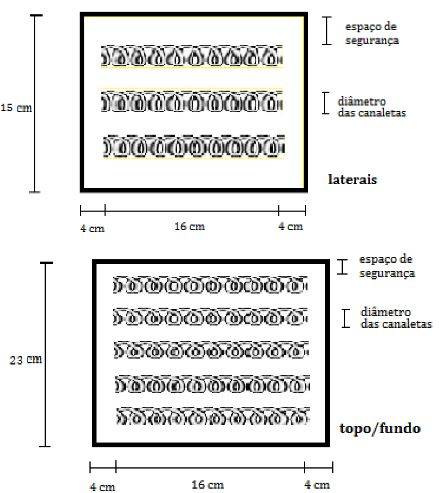
\includegraphics[keepaspectratio=true,scale=1.0]{figuras/alimentacao4.JPG}
\end{figure}

Com 5 canaletas no topo e no fundo e 3 canaletas nas laterais totalizando 16 canaletas com H=16 cm cada. O total de altura da espira é 288 cm.


Com L = 26 metros e H = 2,88 metros, podemos decidir o diâmetro D e o passo h para a melhor distribuição no forno. fazendo h = 0,5 mm entre uma bobina e outra temos uma grande folga entre as bobinas e precisaríamos de um diâmetro da bobina de 1,43 cm, o que é bem razoável para fazer uma canaleta na parede de 5 cm.


Para enrolar as resistências nas especificações dimensionadas usamos um molde de ferro como diâmetro externo e no galpão da FGA (Faculdade Gama) realizamos o procedimento de construção da espira com a barra de ferro de diâmetro = 1,4 cm, tornando a medida do diâmetro externo da espira = diâmetro da canaleta D = 1,56 cm (diâmetro interno + 2 * espessura do fio de 0,18cm). 


Assim obtemos as medidas oficiais da parede do forno utilizando:
\\-o diâmetro das canaletas \textbf{D}; 
\\-o número de espaços \textbf{n}(entre o topo e o fundo e entre as canaletas) ; 
\\-a altura \textbf{h} da parede.

Diâmetro das canaletas = 1,56 cm
\\espaço de segurança nas laterais = *****formula***** = 2,58 cm
\\espaço de segurança na fundo/topo = ****formula**** = 2,53 cm

Os dois espaços de segurança são maiores que 2 cm deixando as resistências bem distribuídas dentro do forno de forma segura e homogênea já que ficarão todas dispostas simetricamente nas paredes em relação às bordas.
As ligações entre uma canaleta a outra serão feitas por um fio não bobinado de resistência aumentando no cálculo do L final cerca de 50 cm de fio ( + $0.25\Omega$)

\begin{figure}[H]
	\centering
	\label{resistencia3}
	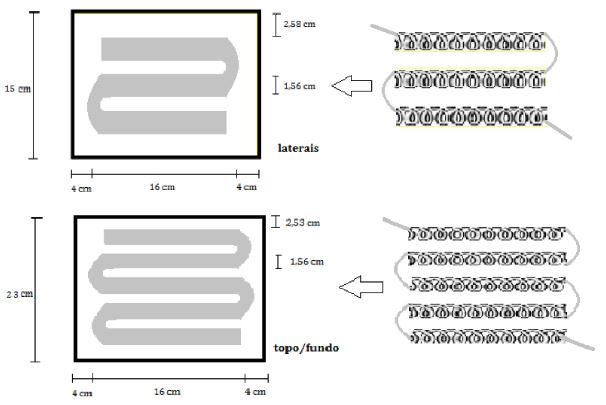
\includegraphics[keepaspectratio=true,scale=1.0]{figuras/alimentacao5.JPG}
\end{figure}

Cada parede tem sua própria espira de resistência, logo as quatro paredes serão ligadas em série e as ligações serão fixadas na parede.

\subsection{Fabricação das espiras resistivas}
Para enrolar as resistências com o material disponível, foi feito um sistema com um cabo de aço de 3,13 metros e diâmetro 1,4cm e dois alicates de pressão. O diâmetro do aço foi o molde para o diâmetro interno da espira. Um alicate de pressão fixou a ponta da resistência no cabo, e outro alicate foi utilizado para girar a barra de aço enquanto o operador tencionava o fio, como no figura abaixo:
\begin{figure}[H]
	\centering
	\label{foto1}
	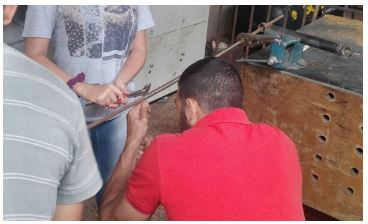
\includegraphics[keepaspectratio=true,scale=1.0]{figuras/alimentacao6.JPG}
\end{figure}

O fio tinha o tamanho \textbf{L} de 28 m e $18\Omega$, a barra tinha a comprimento \textbf{H} de 3,13 m. Com isso conseguimos enrolar a espira de tamanho suficiente para o projeto:
\begin{figure}[H]
	\centering
	\label{foto2}
	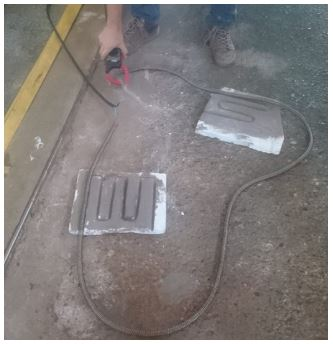
\includegraphics[keepaspectratio=true,scale=1.0]{figuras/alimentacao7.JPG}
\end{figure}

Para a resistência necessária ($15,5 \Omega$) com fator de segurança prático dimensionamos em média 1 Ohm para cada canaleta e recortamos a resistência de cada parede:
\begin{figure}[H]
	\centering
	\label{foto3}
	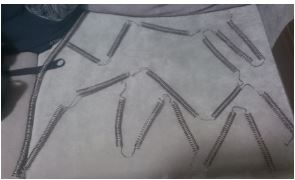
\includegraphics[keepaspectratio=true,scale=1.0]{figuras/alimentacao8.JPG}
\end{figure}

\subsection{Confecção das canaletas na parede do forno}
Para garantir o aquecimento do forno não basta enrolar a espira de resistências, mas precisamos também confeccionar as canaletas em que elas estarão dispostas. Para isso utilizamos o material refratário de 5 cm de espessura e após o lixamento para manter a parede uniforme desenhamos o caminho a ser percorrido pelas canaletas:
\begin{figure}[H]
	\centering
	\label{foto4}
	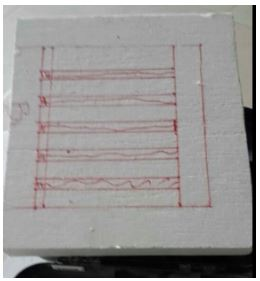
\includegraphics[keepaspectratio=true,scale=1.0]{figuras/alimentacao9.JPG}
\end{figure}

Após todas as marcações concluídas, fizemos as perfurações usando uma furadeira de impacto, tomando o cuidado para perfurar em diagonal nas laterais e no topo para evitar que as canaletas caiam utilizando não somente a pressão, mas também a gravidade para mantê-las dentro da parede como nas figuras:
\begin{figure}[H]
	\centering
	\label{foto5}
	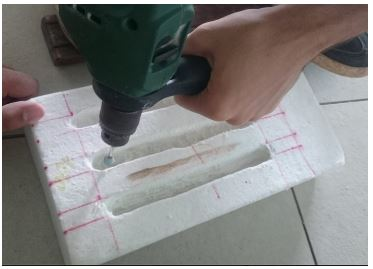
\includegraphics[keepaspectratio=true,scale=1.0]{figuras/alimentacao10.JPG}
\end{figure}

Ajustando os detalhes  mais refinados da canaleta com a lixa e o estilete:
\begin{figure}[H]
	\centering
	\label{foto6}
	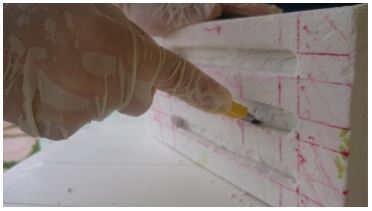
\includegraphics[keepaspectratio=true,scale=1.0]{figuras/alimentacao11.JPG}
\end{figure}

Em testes realizados observamos que a resistência aquecida queima o material refratário. Para resolver o problema revestimos as paredes com cimento, aumentando a pressão quem cima das resistências a serem posicionadas e protegendo a parede do forno de danos causados pela resistência:
\begin{figure}[H]
	\centering
	\label{foto7}
	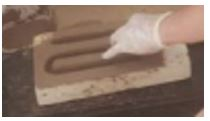
\includegraphics[keepaspectratio=true,scale=1.0]{figuras/alimentacao12.JPG}
\end{figure}

Após a secagem e a instalação das resistências nas canaletas ligadas em série fizemos o circuito de alimentação com as resistências em série direto na tensão da tomada utilizando um fio com capacidade para 3 kW e uma tomada de capacidade de até 20 A. testamos por fim a corrente que passa no sistema com o alicate de medição.
\begin{figure}[H]
	\centering
	\label{foto8}
	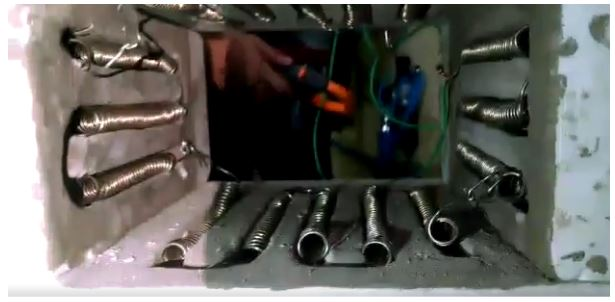
\includegraphics[keepaspectratio=true,scale=1.0]{figuras/alimentacao13.JPG}
\end{figure}

O resultado foi 13,8 A, onde para potência de 3kW é necessário teoricamente uma corrente de 13,6 A, mostrando assim bons resultados práticos. A resistência na teoria tende a aumentar suavemente levando o forno a uma potência um pouco mais baixa a 1200 graus porém com pouca variação como pode ser visto no gráfico TxR. A potência a temperatura ambiente é ***formula**** sendo aproximadamente $R = 15,8 \Omega$, ****formula****, 

Para temperaturas a $1200\degree C$ onde aproximadamente R= 16,2: 
****formula****

Uma diferença desprezível que é possível graças às propriedades do fio que não se alteram bruscamente com o aumento da temperatura.


\subsection{Tratamento Térmico}

Um exemplo de tratamento térmico muito usado na industria é o processo de têmpera, que consiste no submeter o aço a uma temperatura em média 50 ºC acima da zona crítica de austenitização para o aços até 0,8\% de carbono e 50 ºC acima do limite inferior da zona crítica de austenitização para o aços acima de 0,8\% de carbono A zona crítica de austenitização varia com o aumento da composição de carbono no aço como na figura abaixo:
\begin{figure}[H]
	\centering
	\label{austenitizacao}
	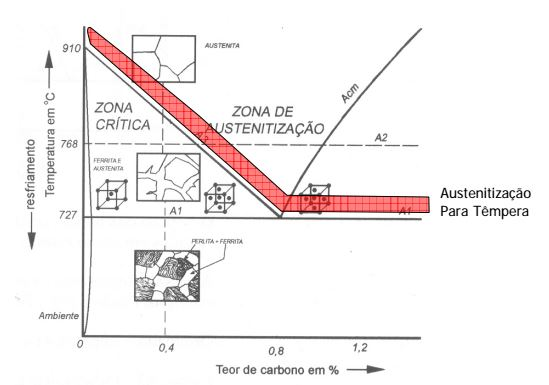
\includegraphics[keepaspectratio=true,scale=0.8]{figuras/austenitizacao.JPG}
	\caption{Zona de Austenitização para Têmpera. Fonte: Tschiptschin}
\end{figure}

Após manter o aço por um tempo  na zona crítica representada pela área vermelha do gráfico, ele muda sua sua estrutura cristalina para a austenítica ou “austenítica + cementita” que a altas temperaturas substituí qualquer estrutura existente no corpo de prova anteriormente.Após esse processo o aço é resfriado bruscamente em água passando de temperaturas entre 780 a 900 graus Celsius à temperatura ambiente de forma rápida com o objetivo de obter a estrutura Martensítica do aço que tem características duras e frágeis e evitando estruturas mais moles como ferrita, bainita e perlita:
\begin{figure}[H]
	\centering
	\label{resfriamento1}
	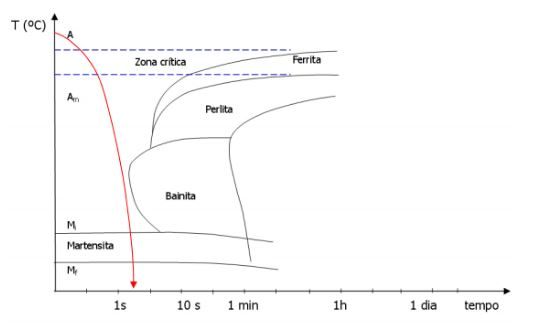
\includegraphics[keepaspectratio=true,scale=0.8]{figuras/resfriamento1.JPG}
	\caption{Resfriamento de temperatura para o processo de têmpera. Fonte: Tschiptschin.}
\end{figure}

O tempo de formação de Martensita é diferente na superfície e no centro do corpo de prova, devido ao contato direto da superfície com o meio refrigerante, levando o tempo da temperização no centro do corpo de prova a ser até 10 vezes maior que na superfície. Essa variação temporal pode gerar diferenças na estrutura do material, e isso deve ser considerado dependendo do objetivo do operador.

\begin{figure}[H]
	\centering
	\label{resfriamento2}
	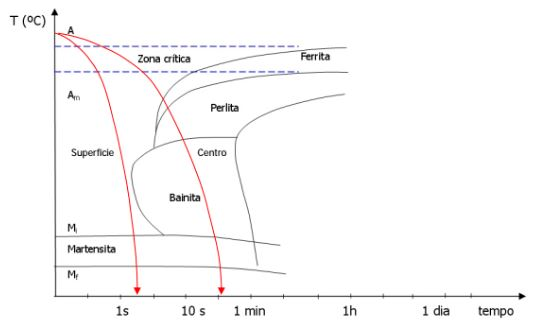
\includegraphics[keepaspectratio=true,scale=0.8]{figuras/resfriamento2.JPG}
	\caption{Resfriamento na superfície no centro do corpo de prova. Fonte: Tschiptschin.}
\end{figure}

\subsection{Material Submetido ao Tratamento}

O aço é definido no Brasil pela NBR 6215:2011 como uma liga ferrosa passível de deformação plástica que, em geral, apresenta teor de carbono entre 0,008\% e 2,0\% na sua forma combinada e, ou, dissolvida e que pode conter elementos de liga adicionados, ou residuais.

No Brasil, a Associação Brasileira de Normas Técnicas - ABTN, por intermédio da norma NBR NM 87:2000 classifica os aços-carbono comuns e os de baixo teor em liga segundo os critérios adotados pela AISI (\textit{American Iron and Steel Institute}) e SAE (\textit{Society of Automotives Engineers}).

\begin{figure}[H]
	\centering
	\label{tab_sae1}
	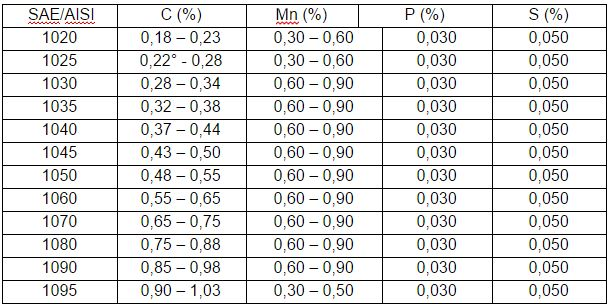
\includegraphics[keepaspectratio=true,scale=0.8]{figuras/tab_sae1.JPG}
	\caption{Composição química de aços Sae 10XX\@. Fonte: ABNT/SAE J403, 1995.}
\end{figure}

\begin{figure}[H]
	\centering
	\label{tab_sae2}
	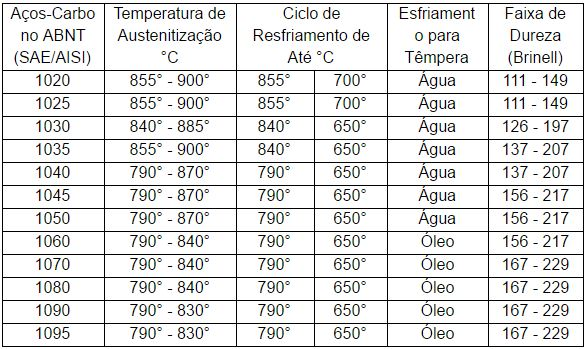
\includegraphics[keepaspectratio=true,scale=0.8]{figuras/tab_sae2.JPG}
	\caption{Características de tratamento térmico de aços-carbono simples.  Fonte: ABNT/SAE J403, 1995.}
\end{figure}

Aços são considerados bons para serem temperados a partir de 40\% de carbono em sua composição, pois possuem resistência suficiente ao desgaste a abrasão e boa tenacidade.

Para o trabalho foi escolhido o corpo de prova SAE 1045, que é considerado aço de médio teor de carbono, por questões de preço, disponibilidade, esfriamento em água facilitado e faixa de dureza próxima à aços com maior porcentagem de carbono.
São aços que possuem boa conformabilidade à frio e razoável resistência mecânica com acabamento laminado, trefilado ou retificado. 

Para que seja realizados tratamentos térmicos, é necessário ter conhecimento sobre a curva TTT (tempo-temperatura-transformação) do material, que relaciona as variáveis da micro estrutura com o tempo e a temperatura.
\begin{figure}[H]
	\centering
	\label{diagramattt}
	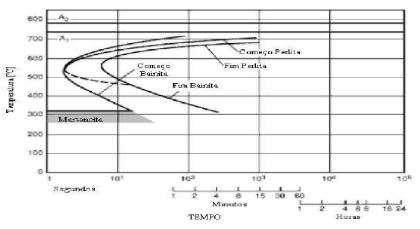
\includegraphics[keepaspectratio=true,scale=0.8]{figuras/diagramattt.JPG}
	\caption{Diagrama TTT do aço SAE 1045 Fonte: DOMINGUES et.al 2010.}
\end{figure}

\begin{figure}[H]
	\centering
	\label{curva_temperatura}
	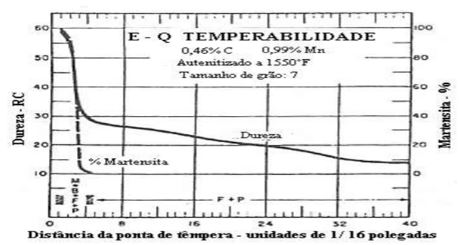
\includegraphics[keepaspectratio=true,scale=0.8]{figuras/curva_temperatura.JPG}
	\caption{Curva de temperabibilidade do aço SAE 1045. Fonte: MARTINS, 2002.}
\end{figure}

O aço Sae 1045 costuma ter no máximo seção transversal de no máximo 60mm. Para seções transversais maiores, o material não apresenta boa reação à têmpera e sua dureza diminui sensivelmente. O aço SAE 1045 deve ser aquecido entre 820ºC e 840ºC em média, por 10 minutos por milímetro, para que haja maior elevação da ductilidade e resistência assim como evitar trincamentos.

O processo de têmpera é completo após a técnica de resfriamento do material, após a temperatura de austenitização, no qual objetiva-se a formação de constituintes resultantes como cementita, ferrita e principalmente martensita, fase metaestável supersaturada de carbono e, portanto de alta dureza. O rápido processo de troca de ambiente de alto calor para um ambiente de baixo calor (até um segundo) permite a formação de martensita.

\begin{figure}[H]
	\centering
	\label{tab_valoresH}
	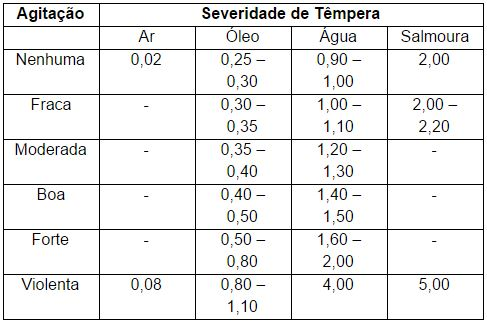
\includegraphics[keepaspectratio=true,scale=0.8]{figuras/tab_valoresH.JPG}
	\caption{Valores de H (coeficientes de severidade de têmpera) para diferentes meios de têmpera. FONTE: SCHEIDEMANTEL, 2014}
\end{figure}

A variação da taxa de resfriamento entre água e salmoura é de 27,6\% até 110\% e a diminuição do tempo de resfriamento é de 7,8\% até 63,3\% em relação à agitação. Ar e óleo possui uma severidade muito baixa de tempera e salmoura possui uam severidade mais alta que o ideal. Dessa forma o resultado de têmpera com resfriamento em água gera um aumento de 20\% de martensita na estrutura do aço em relação á tratamento com salmoura. (CARVALHO, 2004)

\subsection{Resultados}
A estrutura do projeto foi pensada para se obter a menor perda de calor durante o funcionamento do forno, uma variável crítica do projeto, bem como facilidade de fabricação, montagem dos elementos e custo associado.

Portanto uma pesquisa foi realizada pelo grupo elegendo os melhores materiais de acordo com as características do projeto.

\begin{figure}[H]
	\centering
	\label{res1}
	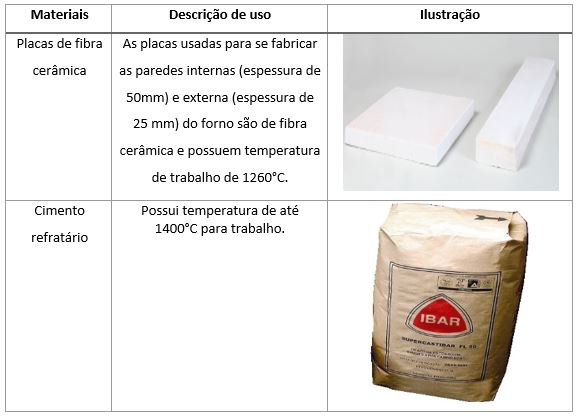
\includegraphics[keepaspectratio=true,scale=0.8]{figuras/res1.JPG}
\end{figure}

 MÉTODOS DE FABRICAÇÃO 
\begin{itemize}
	\item As placas de fibra cerâmicas foram medidas e cortadas de acordo com as dimensões especificadas no projeto segundo a tabela abaixo:
\end{itemize}	
 
\begin{table}[H]
	\centering
	\label{my-label}
	\begin{tabular}{|p{6cm}|p{5cm}|c|}
		\hline
		\textbf{Descrição}                                                                                 & \textbf{Dimensões para produção do forno}                                      & \textbf{Fotos} \\ \hline
		\begin{tabular}[l]{@{}c@{}}Placas laterais de revestimento\\   interno do forno\end{tabular}       & Duas placas com 150 x 310 x 50 mm                                              &               \begin{minipage}{.3\textwidth}
			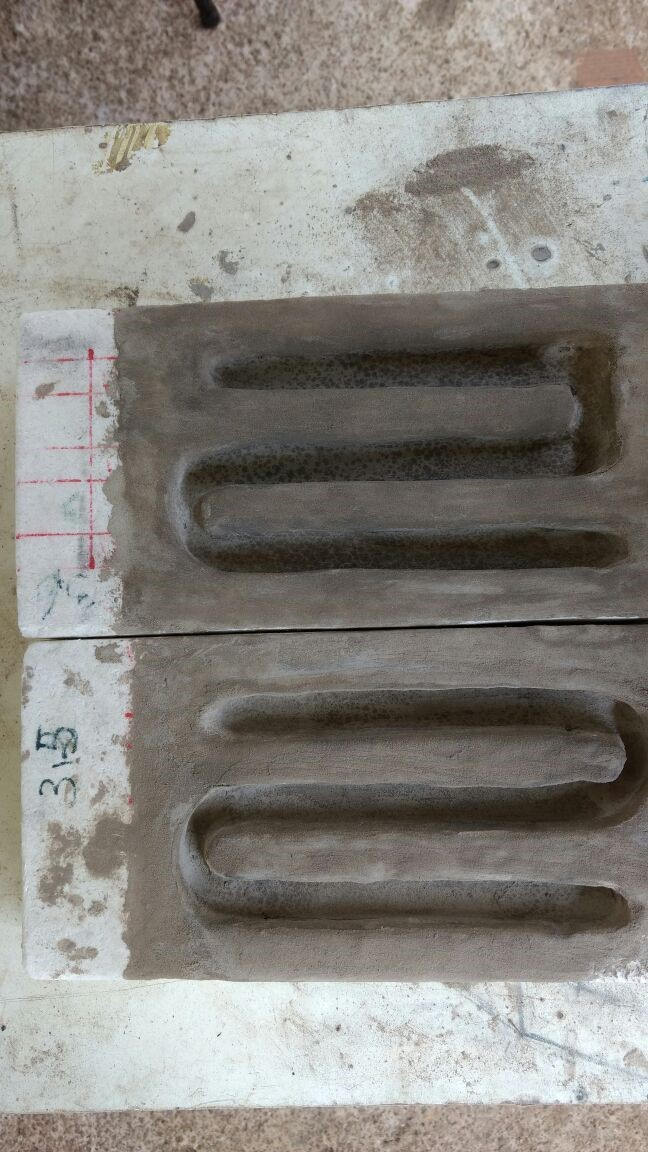
\includegraphics[width=\linewidth, height=50mm]{figuras/3.jpg}
		\end{minipage} \\ \hline
		\begin{tabular}[l]{@{}c@{}}Placas de topo e chão de\\   revestimento interno do forno\end{tabular} & Duas placas com 330 x 310 x 50 mm                                              &                \begin{minipage}{.3\textwidth}
			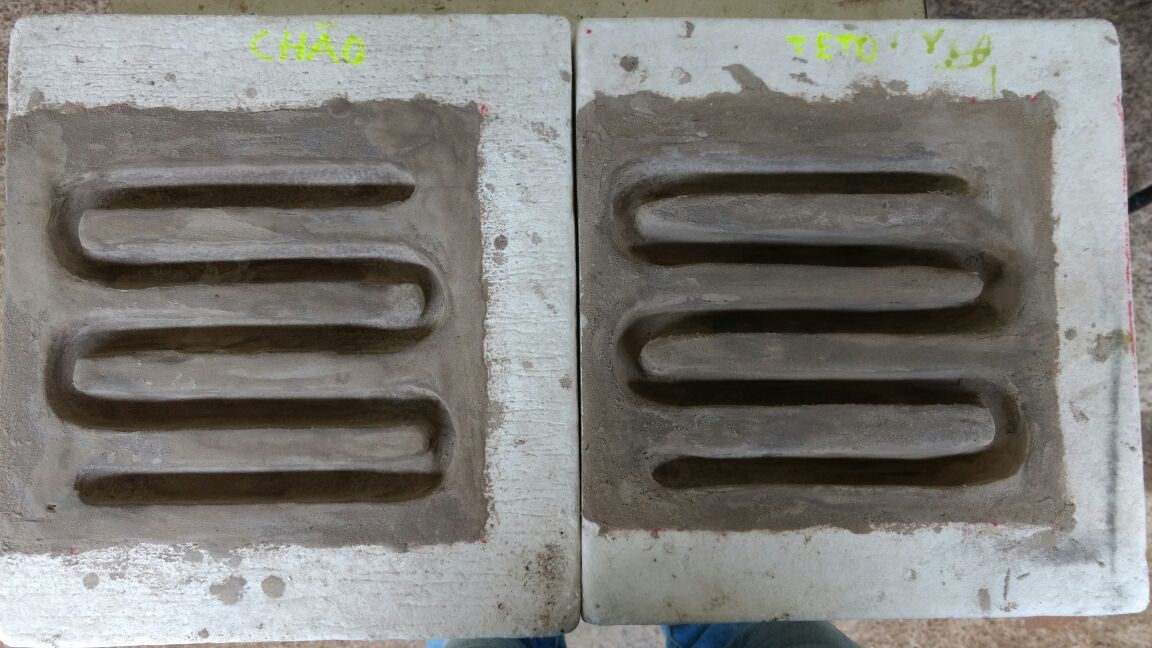
\includegraphics[width=\linewidth, height=35mm]{figuras/4.jpg}
		\end{minipage}\\ \hline
		\begin{tabular}[l]{@{}c@{}}Placa de fundo no revestimento\\   interno do forno\end{tabular}        & Uma placa  230 x 150 x 50 mm                                                   &                \begin{minipage}{.3\textwidth}
			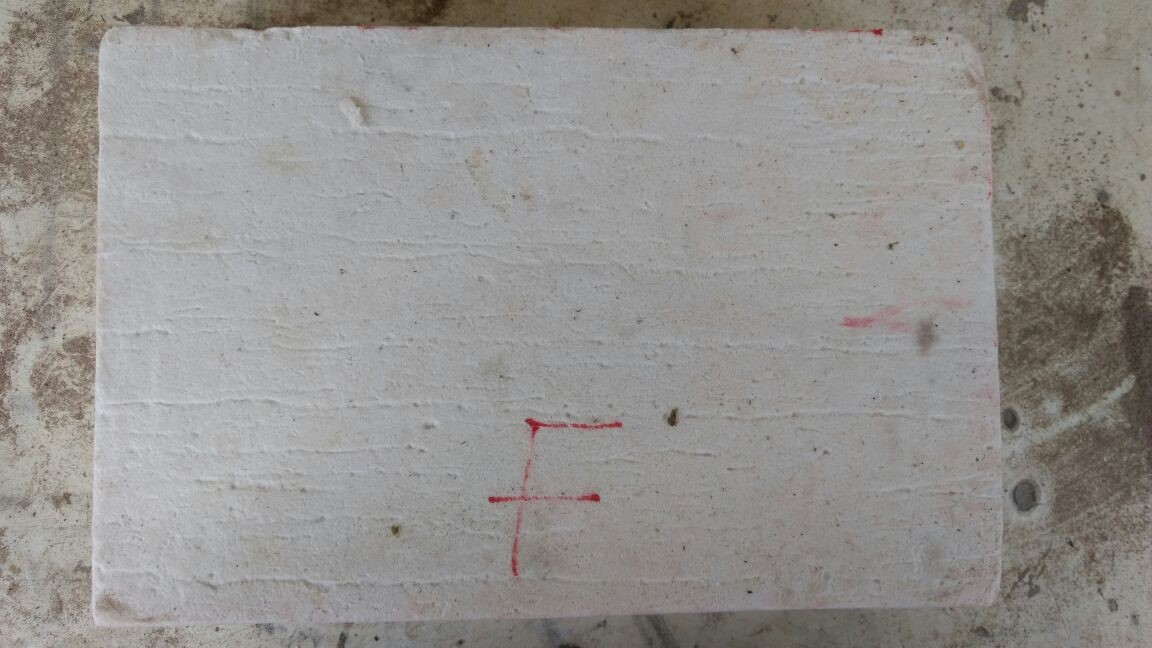
\includegraphics[width=\linewidth, height=35mm]{figuras/5.jpg}
		\end{minipage}\\ \hline
		\begin{tabular}[l]{@{}c@{}}Placa de topo e chao de\\   revestimento externo do forno\end{tabular}  & Duas placas com 480 x 435 x 25 mm                                              &                \begin{minipage}{.3\textwidth}
			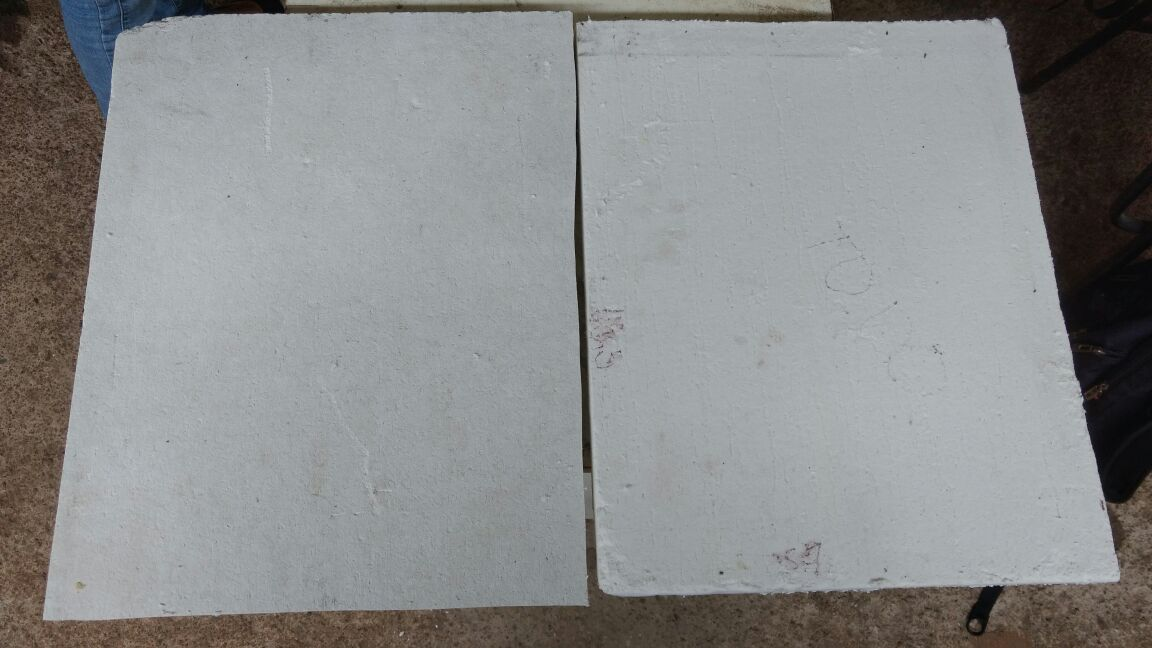
\includegraphics[width=\linewidth, height=35mm]{figuras/6.jpg}
		\end{minipage}\\ \hline
		\begin{tabular}[l]{@{}c@{}}Placas laterais de revestimento\\   externo do forno\end{tabular}       & Duas placas com 480 x 350 x 25 mm                                              &                \begin{minipage}{.3\textwidth}
			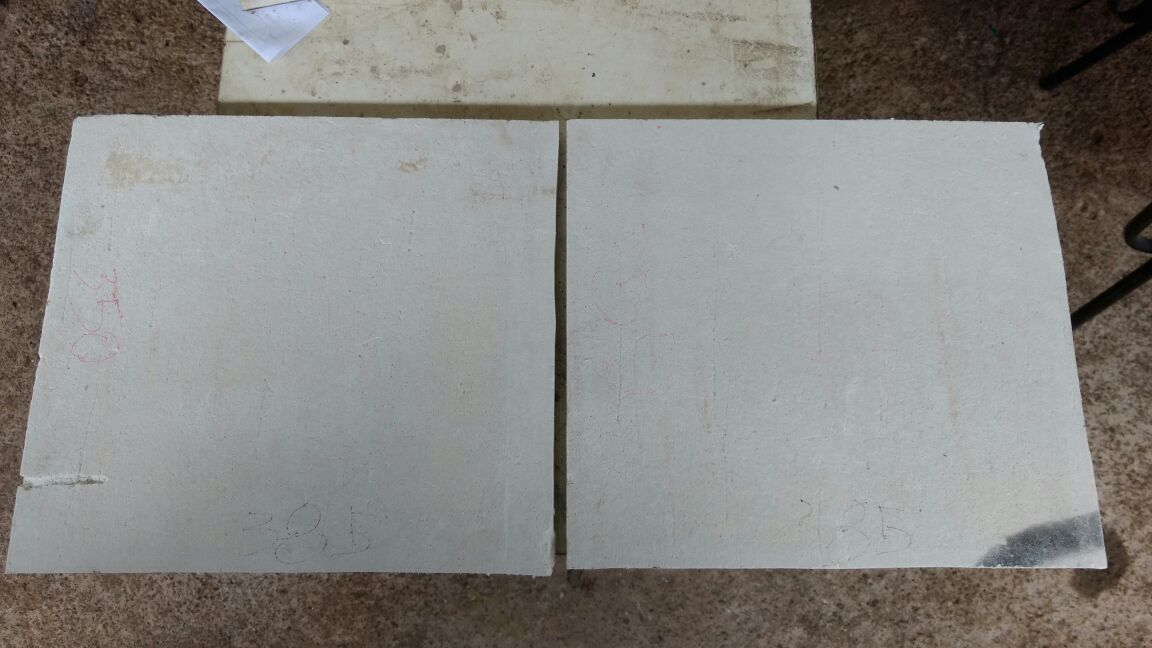
\includegraphics[width=\linewidth, height=35mm]{figuras/7.jpg}
		\end{minipage}\\ \hline
		\begin{tabular}[l]{@{}c@{}}Placa de fundo do revestimento\\   externo do forno\end{tabular}        & \begin{tabular}[c]{@{}c@{}}Uma placa com    430 x 350 x\\   25 mm\end{tabular} &                \begin{minipage}{.3\textwidth}
			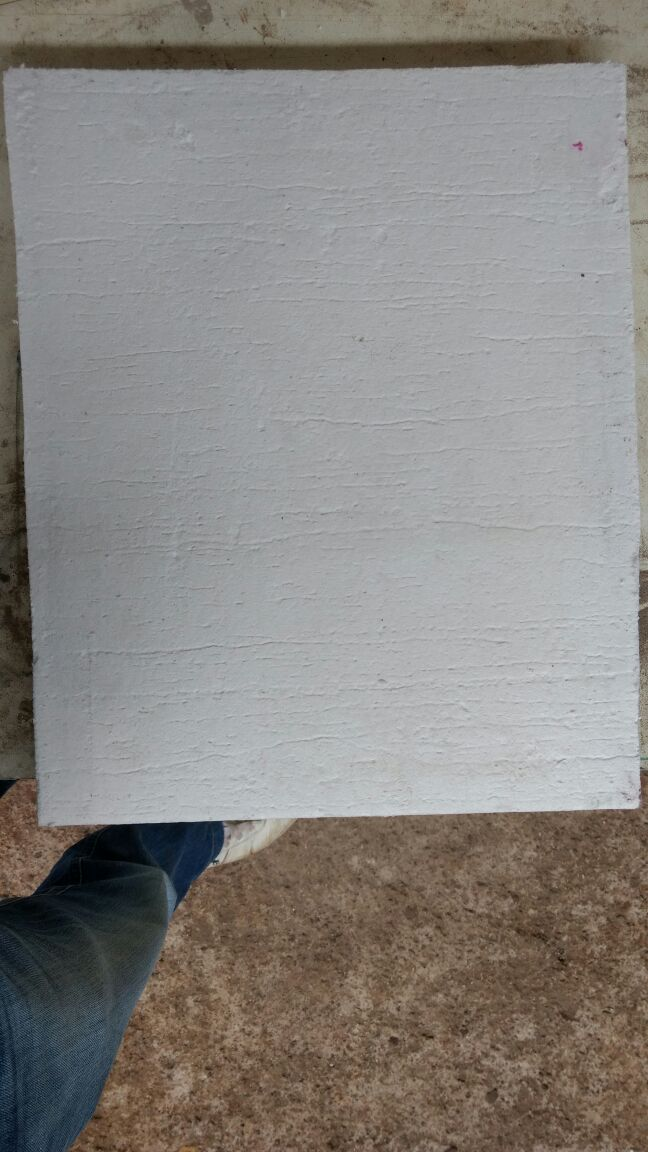
\includegraphics[width=\linewidth, height=50mm]{figuras/8.jpg}
		\end{minipage}\\ \hline
	\end{tabular}
\end{table}

\section{Sistema de Controle}

Para que o forno possa aquecer de maneira controlada, um circuito eletrônico de potência foi desenvolvido para controlar a energia vinda da tomada de 220 V de corrente alternada. O diagrama do sistema pode ser visto na Figura \label{diagramacircuito}.

\begin{figure}[H]
	\centering
	\label{diagramacircuito}
	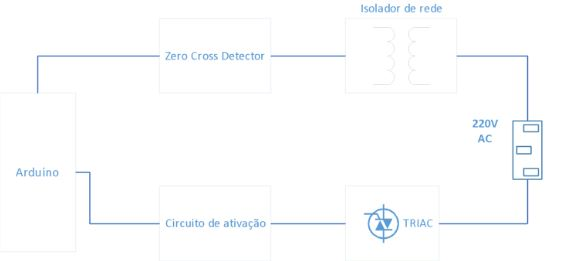
\includegraphics[keepaspectratio=true,scale=1.0]{figuras/diagramacircuito.JPG}
	\caption{Diagrama do circuito de potência}
\end{figure}

\begin{figure}[H]
	\centering
	\label{diagrama}
	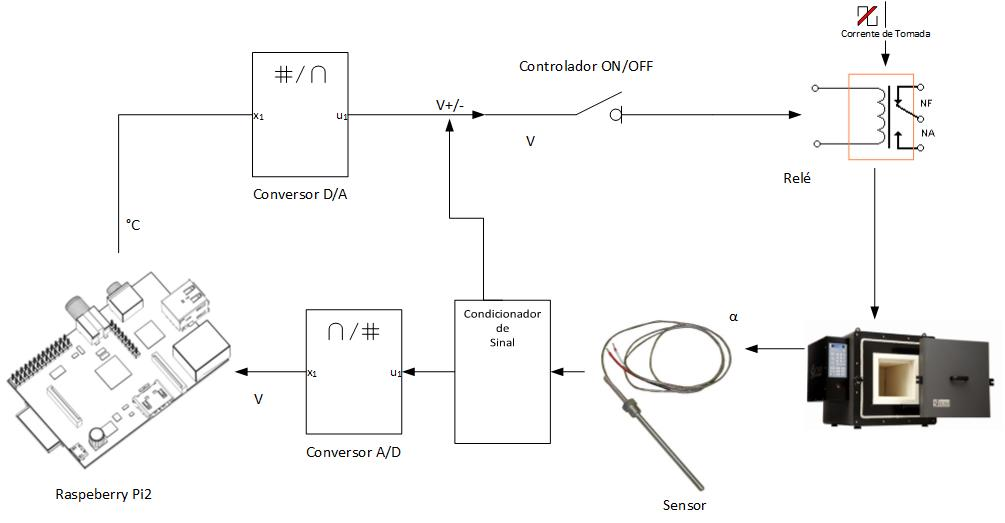
\includegraphics[keepaspectratio=true,scale=0.5]{figuras/diagrama.jpg}
	\caption{Sistema de controle de temperatura do forno}
\end{figure}

Basicamente, o sistema é ligado à um isolador de rede por motivos de segurança que irá diminuir a tensão/corrente e irá se conectar ao detector de passagem por zero. Esse circuito de detecção é responsável por gerar sinais no momento em que a rede cruzar o zero como mostra a Figura \ref{redeAC}. Pelo fato da rede ser de 60Hz, os cruzamentos serão detectados a cada 8.33ms. Esse sinal é então enviado ao microcontrolador arduíno, que irá gerar interrupções durante cada recebimento de cruzamento por zero, e posteriormente, irá executar as funções de tratamento adequada.

\begin{figure}[H]
	\centering
	\label{redeAC}
	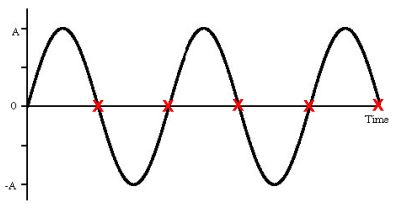
\includegraphics[keepaspectratio=true,scale=1.0]{figuras/redeAC.JPG}
	\caption{Rede AC mostrando os momentos de cruzamento por zero.}
\end{figure}

O arduíno irá então, enviar sinais para o circuito de ativação durante tempos precisamente calculados (da ordem de milisegundos ,o que é totalmente factível para o arduíno, que tem como processador o ATMEGA328 trabalhando a 16MHz).

O circuito de ativação, acionado pelo arduíno, irá então produzir uma corrente de gate necessário para a ativação do triac no tempo calculado. O triac funciona conforme figura \ref{triac}. Ao detectar a passagem por zero, o arduíno irá enviar o sinal para disparar no tempo certo o triac, sendo assim possível controlar a fase de acionamento desse dispositivo. Uma vez acionado, ele só é desligado quando a rede cruza o zero novamente.

\begin{figure}[H]
	\centering
	\label{triac}
	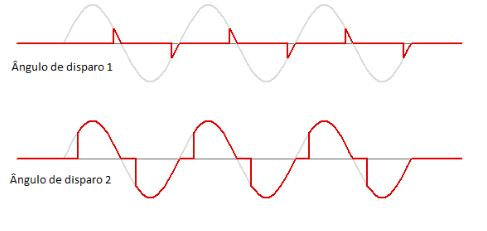
\includegraphics[keepaspectratio=true,scale=1.0]{figuras/triac.JPG}
	\caption{Diferentes ângulos de disparo do triac.}
\end{figure}

O forno foi projetado para funcionar até 14A quando ligado em sua potência máxima. Portanto, foi escolhido o triac BTA41-600b da ST Microelectronics, que suporta correntes de até 40A e transientes de até 400A, dando uma boa margem de segurança para o equipamento.

A figura \ref{circuitocontrole} mostra o circuito completo. Como pode-se ver um transformador 220-18V AC foi utilizado para isolar o circuito da rede. O circuito de detecção por zero é realizado por uma ponte de diodo que irá retificar o sinal, e estará assim, ligando o led contido no optoacoplador 4N25. Esse led polariza o transistor e assim, o arduino consegue detectar os pulsos gerados durante as passagens por zero da rede.

\begin{figure}[H]
	\centering
	\label{circuitocontrole}
	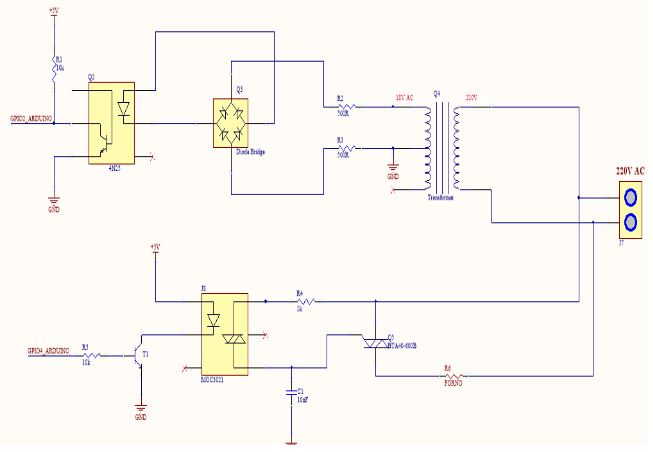
\includegraphics[keepaspectratio=true,scale=1.0]{figuras/circuitocontrole.JPG}
	\caption{Circuito completo de controle.}
\end{figure}

O arduíno envia através do GPIO4 ARDUINO, localizado na parte inferior da figura, os disparos do triac. O MOC3021 é um CI optoacoplador que possui um led e um DIAC. O objetivo desse CI é isolar o arduíno da rede elétrica. Ao mandar um pulso para o transistor T1, esse polariza e deixa passar corrente elétrica, o que liga o LED contido no MOC3021. Esse LED polariza o DIAC contido no CI, que deixa passar uma pequena corrente vinda da rede elétrica. Ao passar a corrente, o TRIAC é ligado, deixando a corrente AC vinda da rede entrar em contato com o forno até o próximo cruzamento por zero. o capacitor C1 é responsável por filtrar eventuais ruídos da rede.

\subsection{Sistema de Temperatura}
O módulo da temperatura é formado por um termopar tipo K que possui faixa de atuação de -270ºC à 1230ºC. Para cada valor de temperatura é gerado uma diferença de potencial de acordo com o anexo 1. Conforme apresentado no diagrama, é necessário um circuito condicionador de sinal, e foi escolhido para isso o CI MAX 6675, que irá amplificar e converter o valor analógico do termopar em um valor digital para leitura da temperatura no Arduíno, além de ser o circuito responsável pela compensação de junção fria, processo necessário para retirar a temperatura ambiente do cálculo da temperatura lida pelo termopar. 

\begin{figure}[H]
	\centering
	\label{termopar}
	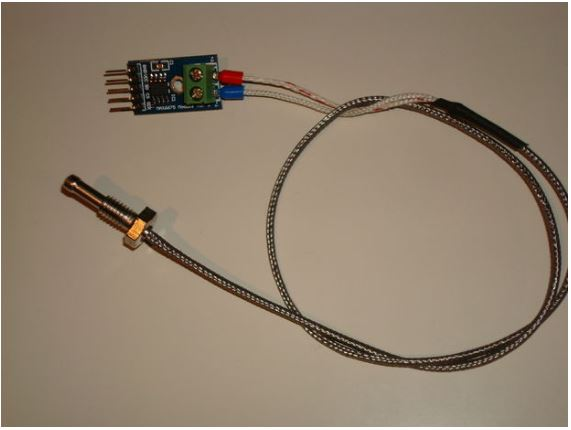
\includegraphics[keepaspectratio=true,scale=1.0]{figuras/termopar.JPG}
	\caption{Termopar com módulo de aquisicação de dados.}
\end{figure}

Para leitura dos dados da temperatura, utiliza-se a biblioteca max6675.h do Arduíno para fazer a comunicação entre o microcontrolador e o termopar através do protocolo SPI (Serial Peripheral Interface). Esse tipo de protocolo é utilizado para a comunicação entre um microntrolador, denominado como mestre, e um ou mais periféricos, denominados como escravos. No ci MAX 6675 o pino SCK deve receber o clock de sincronismo com o Arduíno, o de SO é o pino responsável por enviar os dados de leitura do termopar para o Arduíno e o pino CS indica quando o Arduíno irá requisitar a comunicação com o MAX 6675.

\begin{figure}[H]
	\centering
	\label{datasheet}
	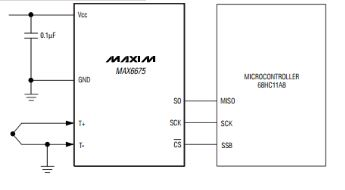
\includegraphics[keepaspectratio=true,scale=1.0]{figuras/datasheet.JPG}
	\caption{Datasheet MAX 6675.}
\end{figure}

\subsection{Controle PID}
Para fazer o controle da temperatura interna do forno será utilizado um controlador PID discreto implementado dentro do Arduíno. O controlador PID é composto por três formas de atuação: proporcional, integral e derivativa. A ação proporcional é responsável por gerar uma resposta mais rápida ao sistema, muitas vezes, quando grande demais, gera instabilidade já que a medida que aumentamos o tempo de resposta da saída aumentamos também o erro do sistema. A ação integral é a correção de erros estacionários que ocorrem ao longo do tempo, nota-se que esta ação não pode ser empregada separada de uma ação proporcional. Por fim, a ação derivativa, assim como a ação integral, não pode ser aplicada separadamente da ação proporcional e tem como objetivo eliminar as variações da saída. Ao juntar as três ações podemos definir um sinal PID como:

*******
formula
*******

Onde:

\begin{itemize}
	\item Kp: Coeficiente da ação proporcional
	\item Ki: Coeficiente da ação integral
	\item Kd: Coeficiente da ação derivativa
	\item E(t): Sinal de erro na entrada do controlador no instante t
	\item u(t): Sinal de controle	
\end{itemize}

Para implementação do PID em um microcontrolador, nota-se pelos sistemas anteriores que precisamos de um controlador digital e para isso o PID deve ser implementado de maneira numérica. Sabendo que as amostras já estarão espaçadas de um mesmo intervalo de tempo muito próximo de zero, pode-se aproximar a integral da equação 1 para uma soma dos dois últimos valores de erro e a derivada para uma subtração. Com isso, a equação discreta do PID que será implementada no Arduíno é:

*******
formula
******

O valor de temperatura recebido via serial pela aplicação web é denominado como set point e comparada com o valor de temperatura mais recente lido pelo termopar chamado de variável de controle. A diferença entre esses dois sinais é chamada de erro, pois é o quanto que falta para a temperatura do nosso sistema, o forno, ser igual a temperatura desejada pelo usuário. Com isso o controlador PID tem a função de tornar o sinal de erro igual a zero.

Através do sinal de erro o controlador PID gera um sinal de controle para o atuador, circuito responsável pelo disparo do dimmer, que consequentemente irá gerar uma ação, seja ela aumentar ou diminuir a potência do forno, que fará o sinal de erro tender a zero. 

\subsection{Trava Eletrônica}
O forno será provido de uma trava controlada eletronicamente por software. Para isso foi escolhido o servo motor TOWER PRO MG995, com possibilidade de movimentação de 180 graus, com torque de 15KG/cm quando alimentado com 5V.  Os testes mostraram que a sua funcionalidade é bem simples, bastando um simples sinal PWM como sinal de controle para a angulação do motor. O circuito está na Figura \ref{trava}:

\begin{figure}[H]
	\centering
	\label{trava}
	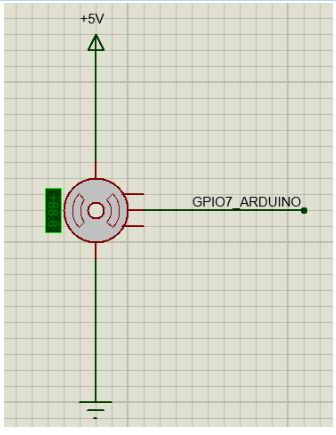
\includegraphics[keepaspectratio=true,scale=0.7]{figuras/trava.JPG}
	\caption{Controle do Servo Motor para trava eletrônica.}
\end{figure}

\subsection{LCD}
O display de LCD 16x02 foi escolhido como interface do forno, para mostrar a temperatura em tempo real em frente ao forno. 

\begin{figure}[H]
	\centering
	\label{lcd}
	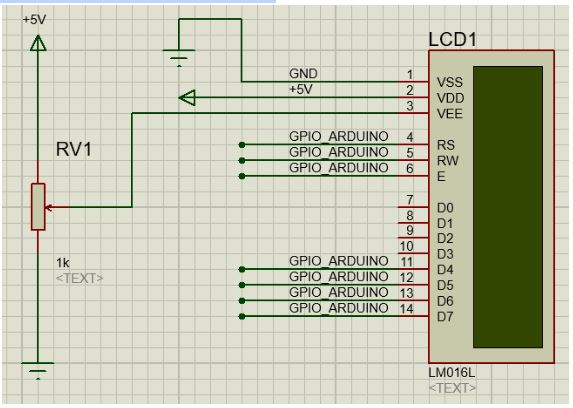
\includegraphics[keepaspectratio=true,scale=0.7]{figuras/lcd.JPG}
	\caption{Controle do Display de LCD.}
\end{figure}

O circuito está na figura \ref{lcd}. Os pinos de escrita e dados são ligados ao arduíno. O potênciômetro é responsável por controlar a luz de fundo do display. A figura X abaixo mostra o display de LCD em funcionamento:

\begin{figure}[H]
	\centering
	\label{display}
	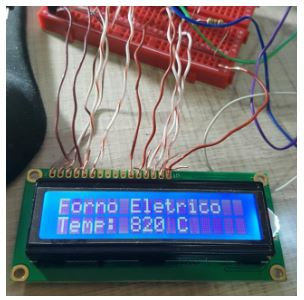
\includegraphics[keepaspectratio=true,scale=1.0]{figuras/display.JPG}
	\caption{Display em Funcionamento.}
\end{figure}

\subsection{Resultados}
Para o teste do controle de potência foi utilizado uma lâmpada incandescente com resistência de $90 \Omega$. Inicialmente foi feito um código, Anexo 1, para reconhecer o cruzamento com zero da rede elétrica e contar quantas vezes isso ocorre por segundo. Para isso, ativa-se uma interrupção no pino 2 do Arduíno e toda vez que esse valor for igual a zero incrementa na variável pulsos. Como esse cruzamento acontece 1 vez a cada meio ciclo e temos uma frequência da senóide da rede elétrica de 60 Hz, o valor reconhecido pelo Arduíno deve ser de 120 conforme imagem abaixo:

\begin{figure}[H]
	\centering
	\label{resultado1}
	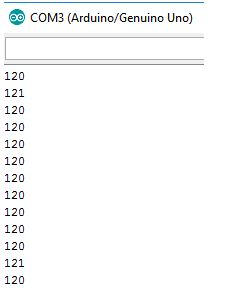
\includegraphics[keepaspectratio=true,scale=1.0]{figuras/resultado1.JPG}
	\caption{Contagem dos cruzamentos por zero de uma rede elétrica de 60 Hz.}
\end{figure}

Ao reconhecer o pulso, deve-se mandar um sinal de ativação do TRIAC de acordo com a quantidade de potência que se deseja inserir na carga, para isso foi feito o código conforme Anexo 2. A tabela a seguir foi feita de acordo com a porcentagem de corrente que se desejava passar para a lâmpada, controlando em qual o ângulo de disparo do triac, e foi medida a tensão de saída da carga:

\begin{figure}[H]
	\centering
	\label{tabpotencia}
	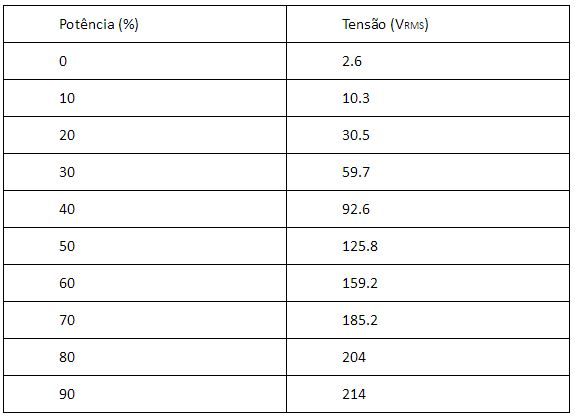
\includegraphics[keepaspectratio=true,scale=1.0]{figuras/tabpotencia.JPG}
	\caption{Relação entre porcentagem da potência desejada e a tensão RMS medida na carga.}
\end{figure}

\begin{figure}[H]
	\centering
	\label{luminosidade}
	\includegraphics[keepaspectratio=true,scale=1.0]{figuras/luminosidade.JPG}
	\caption{Luminosidade da lâmpada x tensão de saída.}
\end{figure}

Para leitura dos valores de temperatura do termopar foi considerado um delay de 1s, conforme mostra o código no Anexo 3, entre as amostras coletadas e apresentado os valores no monitor do Arduíno. Para variar a temperatura foi utilizado um isqueiro próximo ao termopar e visto a temperatura medida.

\begin{figure}[H]
	\centering
	\label{testetemperatura}
	\includegraphics[keepaspectratio=true,scale=1.0]{figuras/testetemperatura.JPG}
	\caption{Teste da temperatura.}
\end{figure}

\section{Arquitetura de Software}

Para a construção da aplicação proposta foi definido a implementação de um sistema web ao qual ficarão dispostas todas as funcionalidades. Este sistema terá como servidor a Raspberry Pi e múltiplos usuários poderão se conectar e visualizar o processo de têmpera.

Com isso, a implementação deste sistema utilizará das seguintes tecnologias:
\begin{itemize}
	\item Linguagem de Programação \textbf{Python} - linguagem de programação de alto nível, multiparadigma, interpretada e de tipagem dinâmica e forte;
	\item \textbf{Django Framework} - framework para desenvolvimento web, escrito em Python, open source, que utiliza o padrão model-template-view. (MTV), utiliza por padrão banco de dados Sqlite3;
	\item \textbf{REST Framework} -  ferramenta open source poderosa e flexível para a construção de APIs Web.
	\item \textbf{ReactJS} - biblioteca open source de JavaScript fornecendo uma visão para os dados processados em HTML. Utiliza-se do conceito de componentes, aos quais permite uma modularização da página web, diminuindo assim sua interdependência e aumentando o reuso.
	
\end{itemize}

\subsection{Metodologia de Desenvolvimento}

A metodologia do projeto de software do forno deverá seguir as seguintes práticas:
\begin{itemize}
	\item Elicitação de requisitos: Serão utilizados métodos de brainstorming e prototipação rápida para aquisição de novas features. Cada feature nova será escrita em um cartão com uma linguagem simples para que qualquer pessoa, sendo desenvolvedora ou não, consiga entender do que se trata. Em cada cartão haverá também valor de prioridade e critérios de aceitação para que o seja validada.
	\item Cartões: os cartões seguem dois modelos. O primeiro, criado em 2001 por uma equipe de desenvolvedores da empresa Connextra. Deve possuir título auto explicativo e a descrição seguindo o formato “Como <papel>, gostaria que <desejo/meta>, de modo que <benefício>”. O segundo é o modelo dos três C’s que foi idealizado por Ron Jeffries também em 2001. Além de conter a descrição do cartão no formato acima, juntamente com o valor de prioridade, ainda há espaços para conversação entre desenvolvedores e clientes e, por fim, os critérios de aceitação que é a confirmação de que o que foi desenvolvido está de acordo com o descrito.
	\item Kanban: ferramenta para indicar o andamento do fluxo do processo de desenvolvimento do software, permite um controle detalhado de em qual etapa se encontra a funcionalidade que esteja sendo desenvolvida. Constitui de um quadro com 4 colunas em geral: Backlog - onde ficam as funcionalidades à serem desenvolvidas; A fazer (To do) - selecionadas as funcionalidades definidas para aquela determinada Sprint, elas são colocadas nesta coluna; Em desenvolvimento (Doing) - funcionalidade em desenvolvimento; Concluída (Done) - após a finalização do desenvolvimento da funcionalidade, esta é posta nesta coluna. Assim sendo, esta ferramenta permite uma visualização melhor do fluxo de trabalho no desenvolvimento da aplicação.
	\item Sprints: é um período de tempo variável entre uma semana a um mês onde as funcionalidades escolhidas são desenvolvidas. No início de cada sprint, uma sprint planning meeting é realizada informalmente para se fazer uma retrospectiva da sprint que passou e planejamento da próxima que está começando.
	
\end{itemize}

\subsection{\textit{Features}}

As features do sistema de controle do forno térmico serão descritas pela matriz Feature e Benefício (FAB) \cite{safe2015}. Elas descrevem os requisitos funcionais do sistema proposto.

\begin{table}[H]
	\raggedright
	\label{my-label}
	\begin{tabular}{|p{3cm}|l|}
		\hline
		\multicolumn{1}{|c|}{\textbf{Features}}                                 & \multicolumn{1}{c|}{\textbf{Benefícios}}                                                                                                                                 \\ \hline
		\begin{tabular}[c]{@{}l@{}}Cadastro de\\   Usuários\end{tabular}        & \begin{tabular}[c]{@{}l@{}}Possibilitar o cadastro de quem\\   poderá utilizar o forno.\end{tabular}                                                                     \\ \hline
		Sistema de Login                                                        & \begin{tabular}[c]{@{}l@{}}Garantir a segurança do sistema,\\   identificando o usuário que utilizará o forno.\end{tabular}                                              \\ \hline
		\begin{tabular}[c]{@{}l@{}}Seletor de\\   Temperatura\end{tabular}      & \begin{tabular}[c]{@{}l@{}}Possibilitar ao usuário escolher a\\   temperatura desejada para a realização do experimento.\end{tabular}                                    \\ \hline
		Cronômetro                                                              & \begin{tabular}[c]{@{}l@{}}Informa o tempo decorrido do\\   experimento, o tempo esperado para término e o tempo restante para \\chegar no   esperado.\end{tabular}      \\ \hline
		\begin{tabular}[c]{@{}l@{}}Gráfico de\\   Temperatura\end{tabular}      & \begin{tabular}[c]{@{}l@{}}Apresentar ao usuário em tempo\\   real a variação de temperatura ocorrida dentro do forno.\end{tabular}                                      \\ \hline
		\begin{tabular}[c]{@{}l@{}}Iniciar\\   Processo de \\Têmpera\end{tabular} & \begin{tabular}[c]{@{}l@{}}Permitir ao usuário iniciar o\\   processo ao que se dará o experimento.\end{tabular}                                                         \\ \hline
		\begin{tabular}[c]{@{}l@{}}Histórico\\   de Sessão\end{tabular}         & \begin{tabular}[c]{@{}l@{}}Salvar relatório dos experimentos\\   anteriormente realizados, e apresentá-los caso solicitados.\end{tabular}                                \\ \hline
		\begin{tabular}[c]{@{}l@{}}Sistema de\\   Segurança\end{tabular}        & \begin{tabular}[c]{@{}l@{}}Dispor de um botão-emergência ao\\   qual deverá interromper o processo imediatamente.\end{tabular}                                           \\ \hline
		Informações                                                             & \begin{tabular}[c]{@{}l@{}}Mostrar informações sobre o\\   processo à de têmpera, assim como as informações necessárias para \\realização do experimento.\end{tabular} \\ \hline
		NBRs                                                                    & \begin{tabular}[c]{@{}l@{}}Apresentar ao usuário as normas\\   relacionadas ao procedimento e materiais.\end{tabular}                                                    \\ \hline
		Estatísticas                                                            & \begin{tabular}[c]{@{}l@{}}Por meio dos dados de experimentos\\   anteriores, apresentar estatísticas sobre a utilização do forno.\end{tabular}                          \\ \hline
	\end{tabular}
	\caption{Matriz de \textit{Features}}
\end{table}

\subsection{Requisitos Implementados (PC2)}
\subsubsection{Cadastro de Usuário}
O sistema de cadastro de usuário que foi implementado necessita das seguintes informações:
\begin{itemize}
	\item User -  é uma chave estrangeira da model de usuários padrão do Django. Possui dados de username, que será a matrícula do usuário, e-mail e senha, que irá variar entre 6 e 16 caracteres.
	\item Nome - primeiro nome do usuário, terá tamanho máximo de 50 caracteres e será obrigatório seu preenchimento;
	\item Sobrenome - sobrenome do usuário, terá tamanho máximo de 50 caracteres e será obrigatório seu preenchimento;
	\item Data de Criação - data ao qual o usuário foi cadastrado, seu preenchimento é automático e pegará a hora e a data atual do sistema;
	\item Matrícula - matrícula do usuário cadastrado, terá tamanho máximo de 10 caracteres e será obrigatório seu preenchimento;
	
\end{itemize}

\subsubsection{Login de Usuário}
Utilizando bibliotecas especiais da tecnologia utilizada, foi implementado o sistema de login/logout e permissões ao qual o usuário irá dispor para o manuseio do sistema e do forno. Os dados necessários para efetuar o login será a matrícula e senha cadastrada.

\subsubsection{Início de Tratamento}
Após o usuário estar autenticado será apresentada a opção de início da realização do experimento, nesta tela será definido os alunos participantes, descrição do material que será tratado, o tempo necessário, a temperatura máxima e o botão de início. Para fim de relatório, o sistema registrará o horário de início e fim do experimento, ou seja, o horário ao qual foi ligado e desligado o forno, e as informações do professor/técnico responsável que estará logado no sistema.

O comando enviado ao arduino será uma string com x caracteres, onde os dois primeiros caracteres definirão o que será acionado. Os dispositivos que serão acionados ao apertar o botão de início serão a corrente que passará pelos resistores para o aquecimento do forno e a trava de segurança da porta por parte de um servomotor. O Arduido, por sua vez, enviará de volta para o servidor uma string com x caracteres informando o valor da corrente e da temperatura, bem como se a porta está trancada.

\subsubsection{Gráfico em Tempo Real}
Iniciado o experimento, o sistema redireciona o usuário para a página de acompanhamento, onde trará as informações de tempo decorrido, temperatura atual do forno por meio de gráfico em tempo real. Este gráfico é responsável por apresentar as informações de temperatura capturada pelo termopar pelo tempo decorrido. Esta página de acompanhado também irá dispor de um botão de segurança para a interrupção do experimento e desligamento do forno.

\subsection{Plano de Teste de Software}
O Plano de Teste de Software é apresentado no Anexo 4.

\section{Mudanças no Escopo}
\subsection{Estrutural}
\subsubsection{Isolamento Térmico}
Na parte estrutural foi a escolhido a utilização das placas cerâmicas no lugar dos tijolos refratários, pela melhor qualidade no isolamento térmico, diminuição de custo e fácil usinabilidade. As características da placa e a sua curva de condutividade térmica estão mostradas abaixo.

\begin{figure}[h]
	\centering
	\label{on_off}
	\includegraphics[keepaspectratio=true,scale=0.8]{figuras/condutividade.JPG}
\end{figure}

Características:
\\Composição: Alumina, Sílica e ligantes
\\Temperatura de trabalho: $1260\degree C$
\\Ponto de fusão: $1750\degree C$
\\Cor padrão: Branca
\\Densidade: $300 Kg/m^{3}$
\\Rigidez dielétrica: 29V/mm

O custo associado a estrutura do forno foi minimizada, pois os tijolos teriam um custo de R\$ 1080,00. Já com as placas refratárias, esse custo foi reduzido pela metade, conforme mostrado no orçamento do fornecedor.  

\begin{figure}[h]
	\centering
	\label{on_off}
	\includegraphics[keepaspectratio=true,scale=0.8]{figuras/custototal.JPG}
\end{figure}

Uma gaxeta para vedação da porta do forno também foi comprada, assim terá uma garantia de menor perda de calor pela mesma.

\subsubsection{Cimento Refratário}
Foi usado para se unir as placas a fim de garantir um isolamento mais satisfatório, e também foi usado como uma camada interna nas placas do forno, pois garante uma resistência mecânica melhor, e o mais importante, resolve o problema de super aquecimento das placas devido ao contato direto com as resistências. De acordo como fornecedor, esse cimento resiste até uma temperatura de $1400\degree C$, que o torna ideal para o uso.
O custo associado a essa mudança foi de 150 R\$, que não foi adicional, pois já iria ser usado para se unir os tijolos especificados no ponto de controle anterior.

\subsection{Sistema de controle}
\subsubsection{Controlador PID}
O controlador inicial sugerido foi o ON/OFF, já que não sabíamos como fazer o controle da corrente que atua sobre a resistência do forno, sendo assim seria feito o controle da temperatura de uma maneira bruta. Porém foi verificado a possibilidade de controlar a potência do forno com o circuito de disparo do dimmer controlando a fase da tensão AC e posteriormente a parcela dessa que atuará sobre a resistência, controlando a temperatura do forno de maneira mais precisa e suave. Esse circuito é chamado de atuador no sistema de controle já que ele irá controlar o comportamento do sistema, o forno. Com a presença de um atuador o controle da solução proposta será feito por um PID já que este é mais seguro, preciso e eficiente do que o controlador ON/OFF.

\subsubsection{Microcontrolador}
Como o circuito que controla a potência do forno é feito no Arduíno, já que este possui saída PWM e permite enviar diferentes sinais de controle, foi unificado todos os códigos, incluindo leitura de temperatura, comunicação com aplicação web e controlador PID, para serem feitos no ambiente do Arduíno. Com isso, a Raspberry Pi não será mais utilizada.

\subsection{Sistema Web}
\subsubsection{Arquitetura de software}
A mudança mais significativa do projeto da aplicação web foi a remoção da ferramenta Django REST Framework (DRF). Esse framework é muito útil para criar APIs (Application Programming Interface) que aceitam requisições de outras aplicação qualquer. A princípio, a ideia de adicionar o DRF era apenas a de incorporar uma nova ferramenta para aumento do escopo do projeto, contudo esta adição não iria agregar valor algum ao produto final. A API que seria criada também não seria útil para nenhuma outra aplicação, pois o produto final ficaria restrito apenas a uma rede local.

Como não há valor agregado, a decisão feita por parte dos desenvolvedores foi de descartar seu uso para evitar um possível \textit{overhead} por desconhecimento da ferramenta e de sua correta implementação.

\subsubsection{Integração}
Como houve mudança na sistema de controle, a integração com este sistema também mudará. Para se comunicar com o Arduino, utilizaremos a biblioteca python chamada pyserial, que faz comunicação com qualquer dispositivo que esteja ligado em uma porta serial. Como o Arduino utilizará uma porta USB (Universal Serial Bus) como fonte de energia para ser ligado, será possível então enviar e receber dados por este meio de transmissão.